\begin{figure}[H]
	\setcounter{subfigure}{0}
	\centering
	\vspace{-1em}	
	\subfloat[切片]{
	\begin{minipage}[t]{0.48\linewidth}
	\centering
	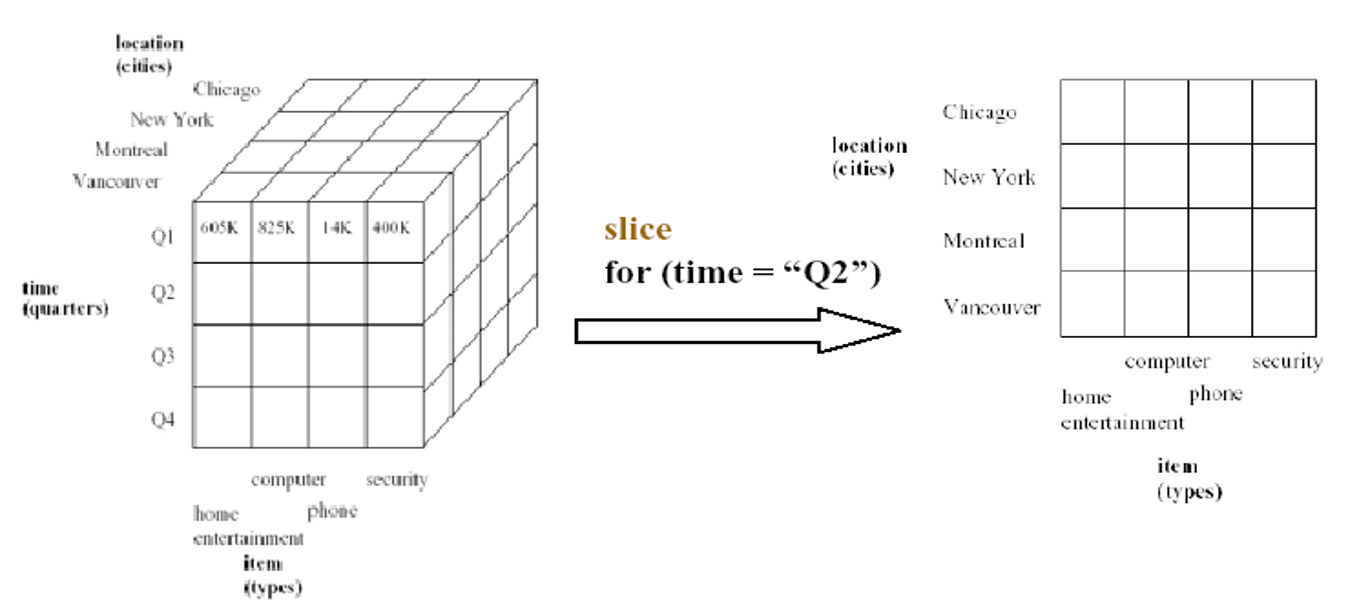
\includegraphics[width=0.97\linewidth]{images/切片.png}
	\end{minipage}
	}
	\subfloat[切块]{
	\begin{minipage}[t]{0.48\linewidth}
	\centering
	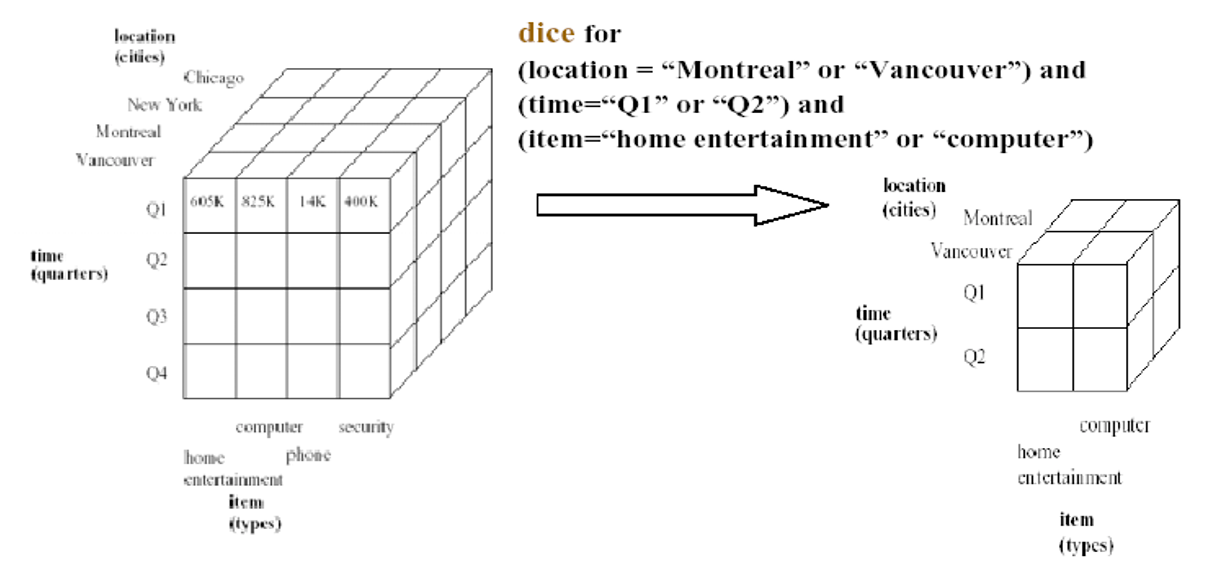
\includegraphics[width=0.97\linewidth]{images/切块.png}
	\end{minipage}
	}

	\subfloat[上钻]{
	\begin{minipage}[t]{0.48\linewidth}
	\centering
	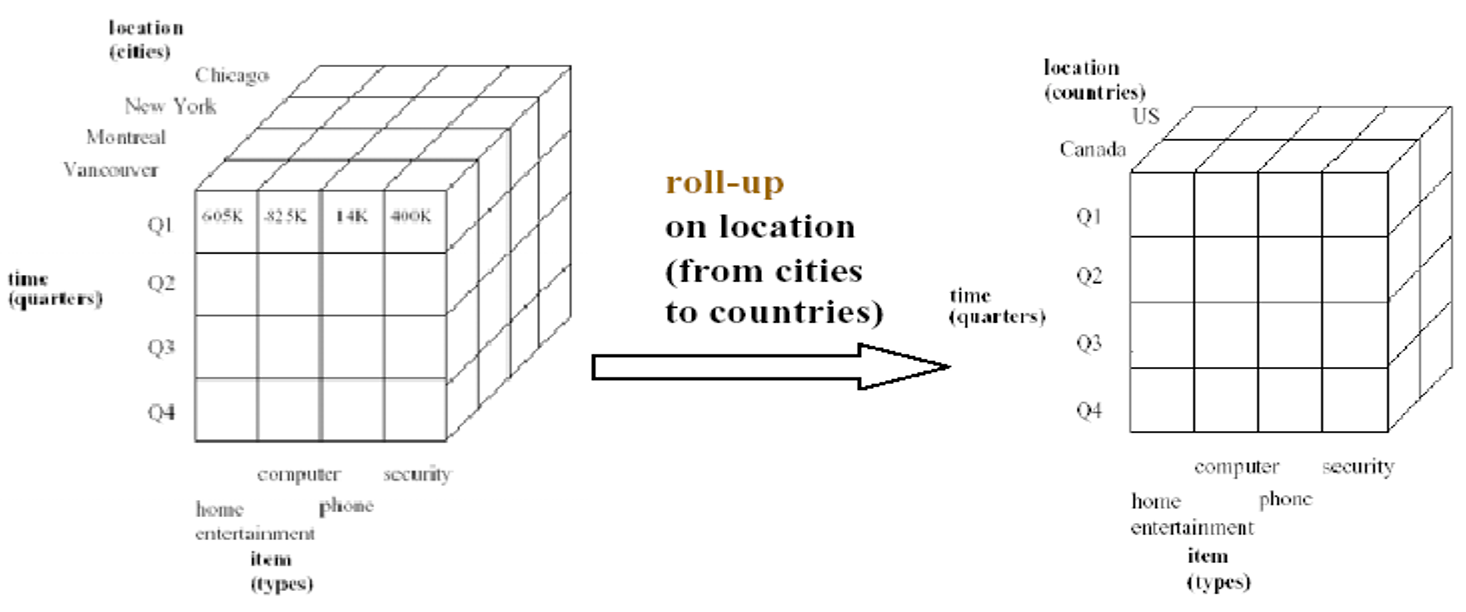
\includegraphics[width=0.97\linewidth]{images/上钻.png}
	\end{minipage}
	}
    \subfloat[下钻]{
	\begin{minipage}[t]{0.48\linewidth}
	\centering
	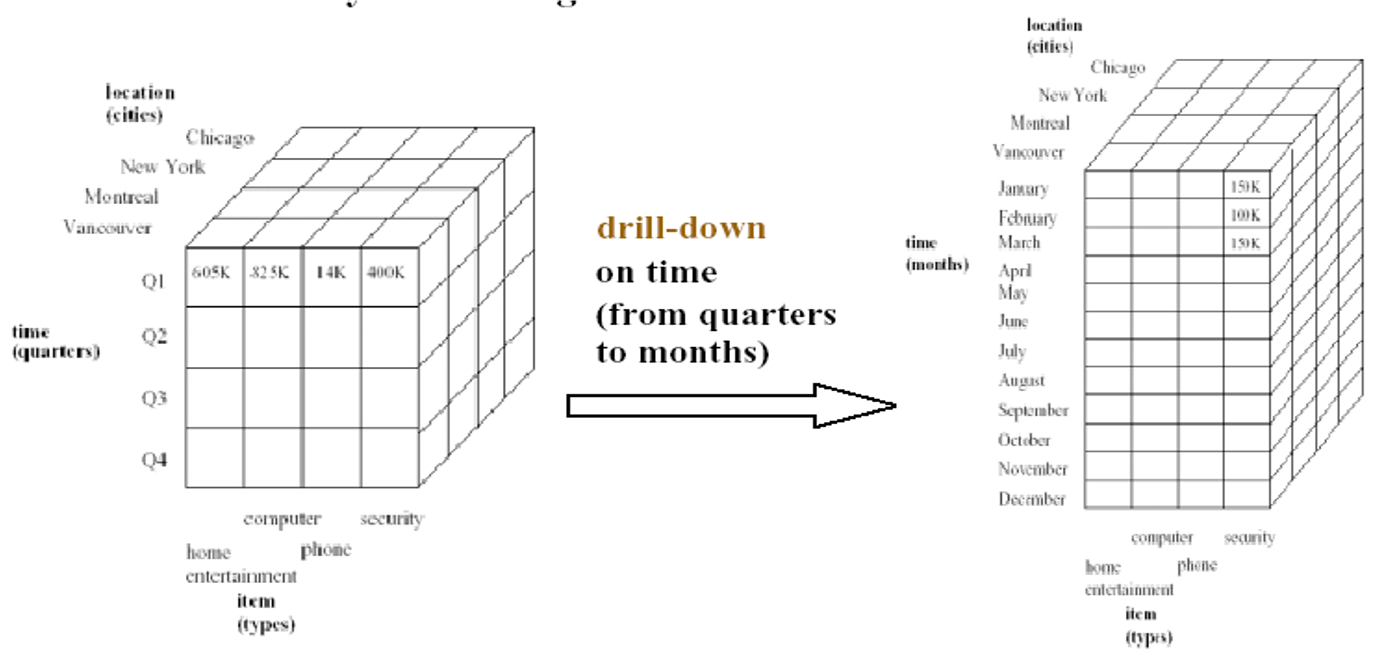
\includegraphics[width=0.97\linewidth]{images/下钻.png}
	\end{minipage}
	}
	\centering
	\vspace{-1.5em}
\end{figure}